
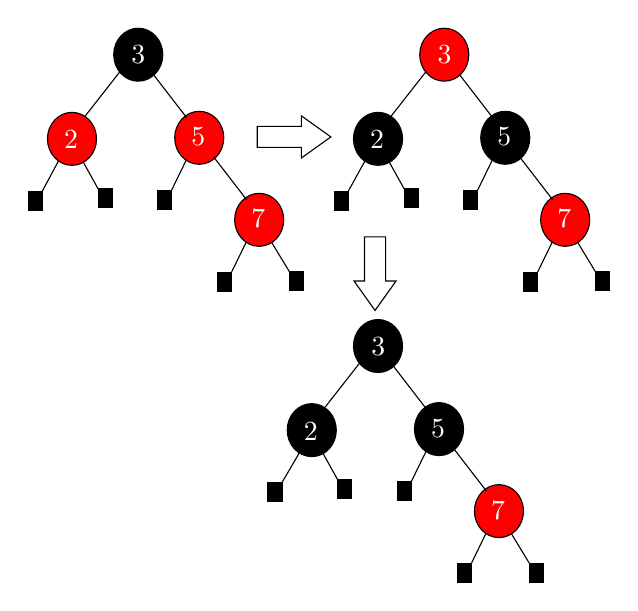
\begin{tikzpicture}[x=0.38pt,y=0.38pt,yscale=-1,xscale=1]
%uncomment if require: \path (0,706); %set diagram left start at 0, and has height of 706

\draw  [fill={rgb, 255:red, 0; green, 0; blue, 0 }  ,fill opacity=1 ]  (48.22, 202.65) rectangle (61.54, 220.61)   ;
\draw    (61.54,202.65) -- (78,172) ;


\draw  [fill={rgb, 255:red, 255; green, 0; blue, 0 }  ,fill opacity=1 ]  (89.83, 152.82) circle [x radius= 23.33, y radius= 25.18]  ;
\draw  [fill={rgb, 255:red, 0; green, 0; blue, 0 }  ,fill opacity=1 ]  (152.83, 72.82) circle [x radius= 23.33, y radius= 25.18]  ;
\draw  [fill={rgb, 255:red, 255; green, 0; blue, 0 }  ,fill opacity=1 ]  (210.83, 151.82) circle [x radius= 23.33, y radius= 25.18]  ;
\draw    (167.5,92) -- (198.83,132.64) ;


\draw  [fill={rgb, 255:red, 0; green, 0; blue, 0 }  ,fill opacity=1 ]  (171.22, 201.65) rectangle (184.54, 219.61)   ;
\draw    (184.54,201.65) -- (198.5,173) ;


\draw    (102.5,131) -- (135.6,88.74) ;


\draw    (100.6,175.01) -- (114.62,200.26) ;


\draw  [fill={rgb, 255:red, 0; green, 0; blue, 0 }  ,fill opacity=1 ]  (114.62, 200.26) rectangle (127.94, 218.22)   ;
\draw    (279.5,251) -- (296.62,279.26) ;


\draw  [fill={rgb, 255:red, 0; green, 0; blue, 0 }  ,fill opacity=1 ]  (296.62, 279.26) rectangle (309.94, 297.22)   ;
\draw  [fill={rgb, 255:red, 255; green, 0; blue, 0 }  ,fill opacity=1 ]  (267.83, 229.82) circle [x radius= 23.33, y radius= 25.18]  ;
\draw    (224.5,170) -- (255.83,210.64) ;


\draw  [fill={rgb, 255:red, 0; green, 0; blue, 0 }  ,fill opacity=1 ]  (228.22, 279.65) rectangle (241.54, 297.61)   ;
\draw    (241.54,279.65) -- (255.5,251) ;


\draw   (266,141) -- (308,141) -- (308,131) -- (336,151) -- (308,171) -- (308,161) -- (266,161) -- cycle ;
\draw  [fill={rgb, 255:red, 0; green, 0; blue, 0 }  ,fill opacity=1 ]  (339.22, 202.65) rectangle (352.54, 220.61)   ;
\draw    (352.54,202.65) -- (370,171) ;


\draw  [fill={rgb, 255:red, 0; green, 0; blue, 0 }  ,fill opacity=1 ]  (380.83, 152.82) circle [x radius= 23.33, y radius= 25.18]  ;
\draw  [fill={rgb, 255:red, 255; green, 0; blue, 0 }  ,fill opacity=1 ]  (443.83, 72.82) circle [x radius= 23.33, y radius= 25.18]  ;
\draw  [fill={rgb, 255:red, 0; green, 0; blue, 0 }  ,fill opacity=1 ]  (501.83, 151.82) circle [x radius= 23.33, y radius= 25.18]  ;
\draw    (458.5,92) -- (489.83,132.64) ;


\draw  [fill={rgb, 255:red, 0; green, 0; blue, 0 }  ,fill opacity=1 ]  (462.22, 201.65) rectangle (475.54, 219.61)   ;
\draw    (475.54,201.65) -- (489.5,173) ;


\draw    (393.5,131) -- (426.6,88.74) ;


\draw    (391.6,175.01) -- (405.62,200.26) ;


\draw  [fill={rgb, 255:red, 0; green, 0; blue, 0 }  ,fill opacity=1 ]  (405.62, 200.26) rectangle (418.94, 218.22)   ;
\draw    (570.5,251) -- (587.62,279.26) ;


\draw  [fill={rgb, 255:red, 0; green, 0; blue, 0 }  ,fill opacity=1 ]  (587.62, 279.26) rectangle (600.94, 297.22)   ;
\draw  [fill={rgb, 255:red, 255; green, 0; blue, 0 }  ,fill opacity=1 ]  (558.83, 229.82) circle [x radius= 23.33, y radius= 25.18]  ;
\draw    (515.5,170) -- (546.83,210.64) ;


\draw  [fill={rgb, 255:red, 0; green, 0; blue, 0 }  ,fill opacity=1 ]  (519.22, 279.65) rectangle (532.54, 297.61)   ;
\draw    (532.54,279.65) -- (546.5,251) ;


\draw   (388,246) -- (388,288) -- (398,288) -- (378,316) -- (358,288) -- (368,288) -- (368,246) -- cycle ;
\draw  [fill={rgb, 255:red, 0; green, 0; blue, 0 }  ,fill opacity=1 ]  (276.22, 479.65) rectangle (289.54, 497.61)   ;
\draw    (289.54,479.65) -- (308,448) ;


\draw  [fill={rgb, 255:red, 0; green, 0; blue, 0 }  ,fill opacity=1 ]  (317.83, 429.82) circle [x radius= 23.33, y radius= 25.18]  ;
\draw  [fill={rgb, 255:red, 0; green, 0; blue, 0 }  ,fill opacity=1 ]  (380.83, 349.82) circle [x radius= 23.33, y radius= 25.18]  ;
\draw  [fill={rgb, 255:red, 0; green, 0; blue, 0 }  ,fill opacity=1 ]  (438.83, 428.82) circle [x radius= 23.33, y radius= 25.18]  ;
\draw    (395.5,369) -- (426.83,409.64) ;


\draw  [fill={rgb, 255:red, 0; green, 0; blue, 0 }  ,fill opacity=1 ]  (399.22, 478.65) rectangle (412.54, 496.61)   ;
\draw    (412.54,478.65) -- (426.5,450) ;


\draw    (330.5,408) -- (363.6,365.74) ;


\draw    (328.6,452.01) -- (342.62,477.26) ;


\draw  [fill={rgb, 255:red, 0; green, 0; blue, 0 }  ,fill opacity=1 ]  (342.62, 477.26) rectangle (355.94, 495.22)   ;
\draw    (507.5,528) -- (524.62,556.26) ;


\draw  [fill={rgb, 255:red, 0; green, 0; blue, 0 }  ,fill opacity=1 ]  (524.62, 556.26) rectangle (537.94, 574.22)   ;
\draw  [fill={rgb, 255:red, 255; green, 0; blue, 0 }  ,fill opacity=1 ]  (495.83, 506.82) circle [x radius= 23.33, y radius= 25.18]  ;
\draw    (452.5,447) -- (483.83,487.64) ;


\draw  [fill={rgb, 255:red, 0; green, 0; blue, 0 }  ,fill opacity=1 ]  (456.22, 556.65) rectangle (469.54, 574.61)   ;
\draw    (469.54,556.65) -- (483.5,528) ;



\draw (89,154) node [color={rgb, 255:red, 255; green, 255; blue, 255 }  ,opacity=1 ] [align=left] {2};
\draw (153,73) node [color={rgb, 255:red, 255; green, 255; blue, 255 }  ,opacity=1 ] [align=left] {3};
\draw (210,151) node [color={rgb, 255:red, 255; green, 255; blue, 255 }  ,opacity=1 ] [align=left] {5};
\draw (267,229) node [color={rgb, 255:red, 255; green, 255; blue, 255 }  ,opacity=1 ] [align=left] {7};
\draw (380,154) node [color={rgb, 255:red, 255; green, 255; blue, 255 }  ,opacity=1 ] [align=left] {2};
\draw (444,73) node [color={rgb, 255:red, 255; green, 255; blue, 255 }  ,opacity=1 ] [align=left] {3};
\draw (501,151) node [color={rgb, 255:red, 255; green, 255; blue, 255 }  ,opacity=1 ] [align=left] {5};
\draw (558,229) node [color={rgb, 255:red, 255; green, 255; blue, 255 }  ,opacity=1 ] [align=left] {7};
\draw (317,431) node [color={rgb, 255:red, 255; green, 255; blue, 255 }  ,opacity=1 ] [align=left] {2};
\draw (381,350) node [color={rgb, 255:red, 255; green, 255; blue, 255 }  ,opacity=1 ] [align=left] {3};
\draw (438,428) node [color={rgb, 255:red, 255; green, 255; blue, 255 }  ,opacity=1 ] [align=left] {5};
\draw (495,506) node [color={rgb, 255:red, 255; green, 255; blue, 255 }  ,opacity=1 ] [align=left] {7};


\end{tikzpicture}